% Build from this folder after running the notebook:
%   rsvg-convert -f pdf ../figures/prediction/sub-03-lags.svg -o ../figures/prediction/sub-03-lags.pdf
%   rsvg-convert -f pdf ../figures/prediction/sub-03-window-brainmap.svg -o ../figures/prediction/sub-03-window-brainmap.pdf
%   pdflatex prediction.tex && pdflatex prediction.tex
\documentclass[11pt]{article}
\usepackage[margin=1in]{geometry}
\usepackage[T1]{fontenc}
\usepackage{lmodern}
\usepackage{microtype}
\usepackage{graphicx}
\usepackage{booktabs}
\usepackage{caption}
\usepackage[hidelinks]{hyperref}

\graphicspath{{../figures/prediction/}}
\captionsetup{font=small, labelfont=bf}

\title{Encoding performance for predicted and unpredicted words in sub-03}
\author{DeepBrain, Podcast ECoG reproduction}
\date{17 November 2026}

\begin{document}
\maketitle

\section*{Summary}

We fit the GPT-2 XL (layer 24) encoding model from \texttt{code/encoding.py} to sub-03 and scored its held-out predictions separately on words that GPT-2 XL predicted and words it did not, after matching the two groups on word frequency and spoken duration. Averaged over the 185 significant electrodes, both groups were encoded at similar levels across lags, with peak correlations of $r = 0.040$ at 0.53\,s for predicted words and $r = 0.038$ at 0.25\,s for unpredicted words. In the second before word onset, encoding performance was slightly lower for predicted words (mean difference $-0.0023$), and the sign of the difference split almost evenly across electrodes (94 of 185 positive). These numbers describe one subject and are not a statistical test.

\section{Methods}

\paragraph{Word groups.}
We used the 5,136 words with an onset in the GPT-2 XL transcript shipped with the dataset (\texttt{stimuli/gpt2-xl/transcript.tsv}). A word counts as predicted when the GPT-2 XL rank of its first token is 0, that is, when the model's highest-probability next token at word onset was the actual token. This gave 1,485 predicted words (28.9\%) and 3,651 unpredicted words. Word frequency is the Zipf frequency from wordfreq 3.1.1, computed after removing punctuation and lowercasing. Words not in wordfreq get 0. There are 13 of these: 8 proper-noun tokens (e.g., ``Dhuey''), 2 occurrences of ``redressability'', and 3 compounds that the transcript spells without hyphens (e.g., ``selfpublishing''). Spoken duration is the end of a word's last token minus its onset.

\paragraph{Encoding model.}
The model is the one in \texttt{code/encoding.py}, unchanged. GPT-2 XL layer-24 embeddings were averaged within each word, the high-gamma signal of all 235 good ECoG electrodes was epoched from $-2$ to $+2$\,s around word onset and resampled to 32\,Hz (128 lags), and electrode-wise ridge regression was fit with the ridge penalty chosen by inner five-fold cross-validation, inside an outer two-fold cross-validation without shuffling. Epoching kept 5,130 words (1,484 predicted, 3,646 unpredicted). The encoding performance on all held-out words is identical to the output of \texttt{code/encoding.py} (maximum absolute difference 0).

\paragraph{Matched subsampling.}
Within each test fold, we binned words by Zipf frequency (bins of 0.5) and by duration (quartiles over all words). In every bin, we drew the same number of predicted and unpredicted words without replacement, then correlated the model-predicted and actual activity over each group's words at every electrode and lag. We repeated the draw 200 times (seed 0) and averaged the group scores over the two folds.

\paragraph{Electrode selection.}
We used the same test as the paper on the encoding performance for all held-out words: each electrode's maximum over lags was compared with a null of 10,000 correlations between random Gaussian vectors of length 2,384 (seed 0), with one-sided p-values and Benjamini-Hochberg false discovery rate (FDR) correction at 0.01. This left 185 of 235 electrodes.

\section{Results}

\paragraph{Matching.}
Each matched sample held 692 words per group in the first fold and 737 in the second, 1,429 per group in total. After matching, the group means differed by 0.008 Zipf and 0.13\,ms (Table~\ref{tab:groups}). Every sample kept 1,429 of the 1,484 predicted words (96\%) and drew the unpredicted words from the frequent, short end of that group, so the matched comparison is between nearly all predicted words and a frequency- and duration-matched subset of unpredicted words.

\begin{table}[htbp]
\centering
\caption{Word groups before and after matching. After-matching values are means over 200 iterations; word counts are summed over the two test folds.}
\label{tab:groups}
\begin{tabular}{lrrrrrr}
\toprule
 & \multicolumn{3}{c}{Before matching} & \multicolumn{3}{c}{After matching} \\
\cmidrule(lr){2-4} \cmidrule(lr){5-7}
Group & Words & Zipf & Duration (s) & Words & Zipf & Duration (s) \\
\midrule
Predicted   & 1,484 & 6.372 & 0.191 & 1,429 & 6.330 & 0.1948 \\
Unpredicted & 3,646 & 5.648 & 0.248 & 1,429 & 6.322 & 0.1946 \\
\bottomrule
\end{tabular}
\end{table}

\paragraph{Encoding performance across lags.}
Both groups showed the temporal profile of the all-word model, rising before word onset and peaking after it (Figure~\ref{fig:lags}). The all-word curve over the same electrodes peaks at 0.25\,s with $r = 0.039$. The predicted-word curve peaks later, at 0.53\,s ($r = 0.040$), and the unpredicted-word curve peaks at 0.25\,s ($r = 0.038$). The unpredicted-word curve reaches nearly the same value at 0.59\,s ($r = 0.037$), a gap of 0.001, which is smaller than the typical change between adjacent lags from 0 to 1\,s (0.002 for either curve). We therefore do not interpret the difference in peak lag.

\begin{figure}[htbp]
\centering
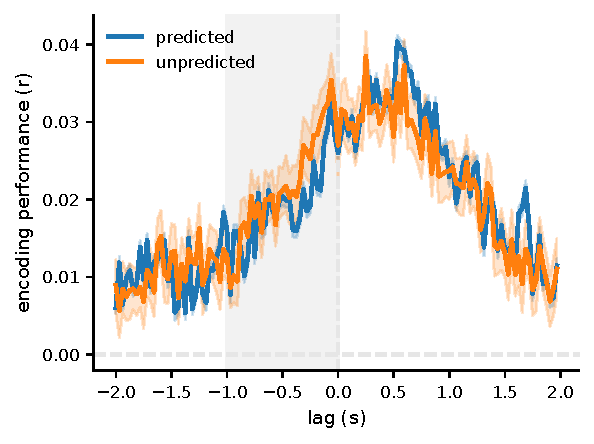
\includegraphics[width=0.6\textwidth]{sub-03-lags.pdf}
\caption{Encoding performance for predicted (blue) and unpredicted (orange) words, averaged over the 185 significant electrodes. Lines are means over 200 matched iterations; bands span the 2.5th to 97.5th percentile across iterations. The gray area marks $-1$ to 0\,s.}
\label{fig:lags}
\end{figure}

\paragraph{Before word onset.}
In the window from $-1$ to 0\,s (32 lags), mean encoding performance over significant electrodes was $r = 0.0191$ for predicted words and $r = 0.0214$ for unpredicted words. The difference was $-0.0023$, with 95\% of iterations between $-0.0039$ and $-0.0010$, and none of the 200 iterations was above 0. Per electrode, 94 of 185 significant electrodes had a positive difference, and differences ranged from $-0.062$ to $0.022$ (Table~\ref{tab:summary}, Figure~\ref{fig:brainmap}). The largest negative differences fall near the Sylvian fissure in the lateral projections. We did not assign these electrodes to regions here.

\begin{figure}[htbp]
\centering
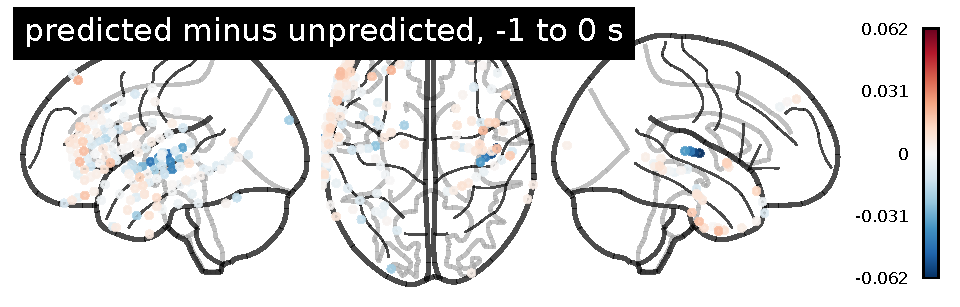
\includegraphics[width=\textwidth]{sub-03-window-brainmap.pdf}
\caption{Difference in mean encoding performance from $-1$ to 0\,s (predicted minus unpredicted), averaged over iterations, for the 185 significant electrodes.}
\label{fig:brainmap}
\end{figure}

\begin{table}[htbp]
\centering
\caption{Summary of the sub-03 results.}
\label{tab:summary}
\begin{tabular}{lr}
\toprule
Quantity & Value \\
\midrule
Predicted and unpredicted words after epoching & 1,484 and 3,646 \\
Matched words per group, fold 1 and fold 2 & 692 and 737 \\
Matched mean Zipf, predicted and unpredicted & 6.330 and 6.322 \\
Matched mean duration (s), predicted and unpredicted & 0.1948 and 0.1946 \\
Significant electrodes & 185 of 235 \\
Electrodes with a positive $-1$ to 0\,s difference & 94 of 185 \\
Iterations with a positive electrode-averaged difference & 0 of 200 (0.0\%) \\
Peak of predicted-word curve & $r = 0.040$ at 0.531\,s \\
Peak of unpredicted-word curve & $r = 0.038$ at 0.250\,s \\
\bottomrule
\end{tabular}
\end{table}

\section{Limitations}

\begin{enumerate}
\item These results come from one subject and include no test of the group difference. The next step compares the difference against a null distribution that preserves the autocorrelation of the neural signal.
\item The spread across iterations reflects only which words are drawn. Because nearly all predicted words appear in every draw, the predicted-word band in Figure~\ref{fig:lags} is narrow and the unpredicted-word band carries most of the spread. Neither band includes noise in the neural data or the autocorrelation of the signal and the embeddings, so the 0 of 200 count should not be read as a p-value.
\item Each matched sample uses about 700 words per fold, roughly a quarter of the test fold, so the group correlations are noisier than the all-word scores.
\item Contextual embeddings can encode activity before word onset through their correlation with the embeddings of preceding words. This analysis does not control for that.
\item Goldstein et al. (2022) reported higher pre-onset encoding for words GPT-2 predicted correctly, using non-contextual (GloVe) embeddings. We used contextual embeddings, so the two results are not directly comparable, and the small difference here runs in the opposite direction.
\end{enumerate}

\section{Reproducing}

The run used the CPU (himalaya numpy backend) with mne 1.13.2, mne-bids 0.20.0, himalaya 0.4.11, nilearn 0.14.1, and wordfreq 3.1.1. \texttt{make prediction} took 8.5\,min with a peak memory of 5.9\,GB and wrote a 48\,MB result file.

\begin{verbatim}
python code/download.py --subjects 03 --features gpt2-xl
python code/encoding.py --modelname=gpt2-xl --layer=24 --subject=03
make prediction
jupyter nbconvert --to notebook --inplace --execute notebooks/prediction.ipynb
\end{verbatim}

\noindent The script writes
\begin{verbatim}
results/sub-03/prediction/sub-03_task-podcast_desc-gpt2.xl.l24_result.h5
\end{verbatim}
and the notebook saves the figures to \path{figures/prediction/}.

\end{document}
